\chapter{Appendix}


\begin{figure}[htbp]
    % \ContinuedFloat
	\centering
	\begin{subfigure}[t]{0.8\textwidth}
		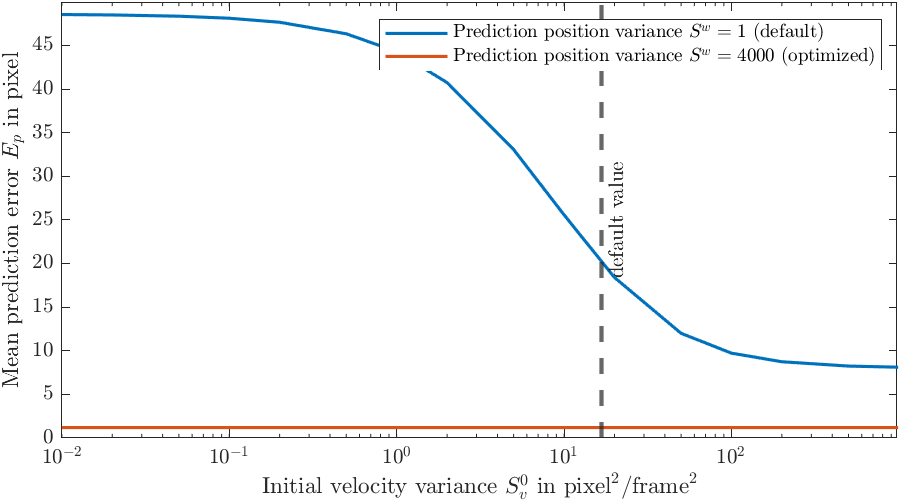
\includegraphics[width=\textwidth]{figures/KF/appendix/iniv cv.png} 
		\caption{Initial velocity variance $S_{\mathrm{vel}}^{\mathrm{ini}}$ in CV model.}
	\end{subfigure}
	\vskip\baselineskip
	\quad
	\begin{subfigure}[t]{0.8\textwidth}
		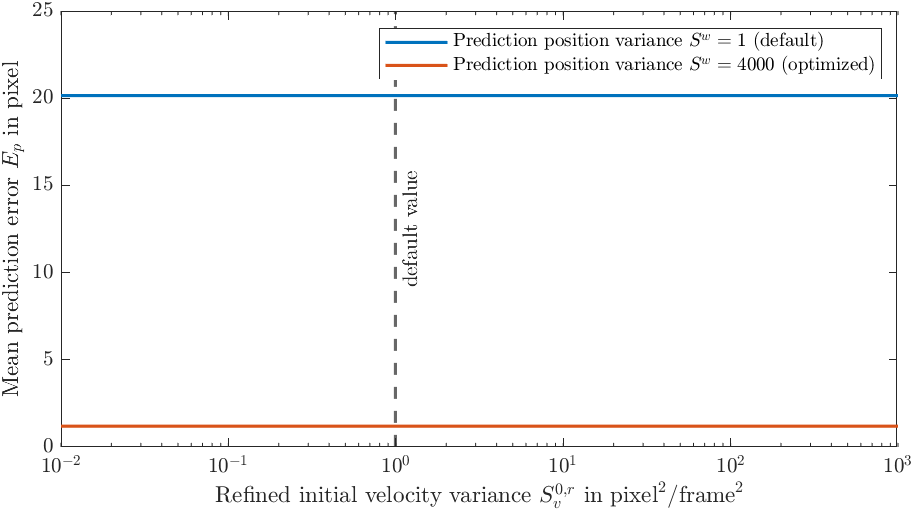
\includegraphics[width=\textwidth]{figures/KF/appendix/inirv cv.png}
		\caption{Refined initial velocity variance $S_{\mathrm{vel}}^{0,r}$ in CV model.}
	\end{subfigure}
	\caption{The grid search result of $S_{\mathrm{vel}}^{\mathrm{ini}}$ and $S_{\mathrm{vel}}^{0,r}$ in CV model when the system noise power spectral density $S^{\boldmath{w}}$  is set as default or optimized value.}
	\label{grid search cv appendix}
\end{figure}

\begin{figure}
    % \ContinuedFloat
    \centering
	\begin{subfigure}[t]{0.8\textwidth}
		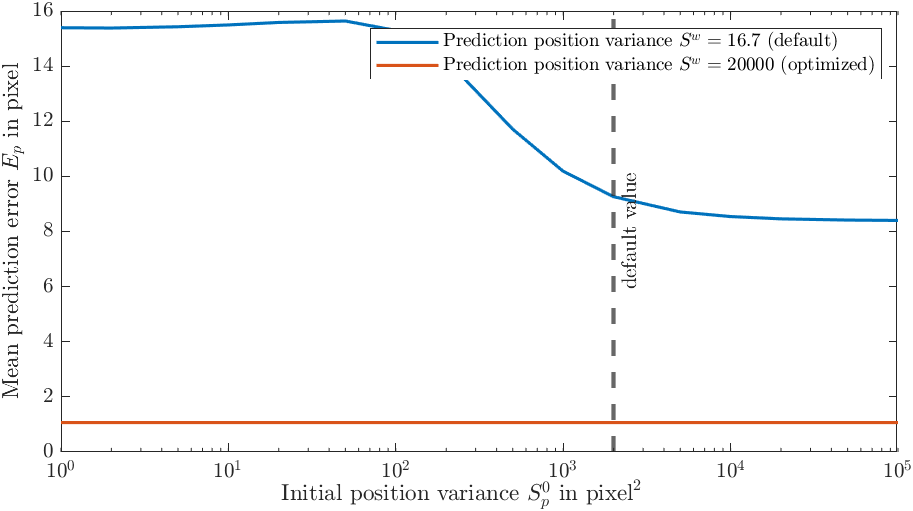
\includegraphics[width=\textwidth]{figures/KF/appendix/inip cva.png}
		\caption{Initial position noise power spectral density $S_{\mathrm{pos}}^{\mathrm{ini}}$ in CVA model.}
	\end{subfigure}
% 	\vskip\baselineskip
	\begin{subfigure}[t]{0.8\textwidth}
		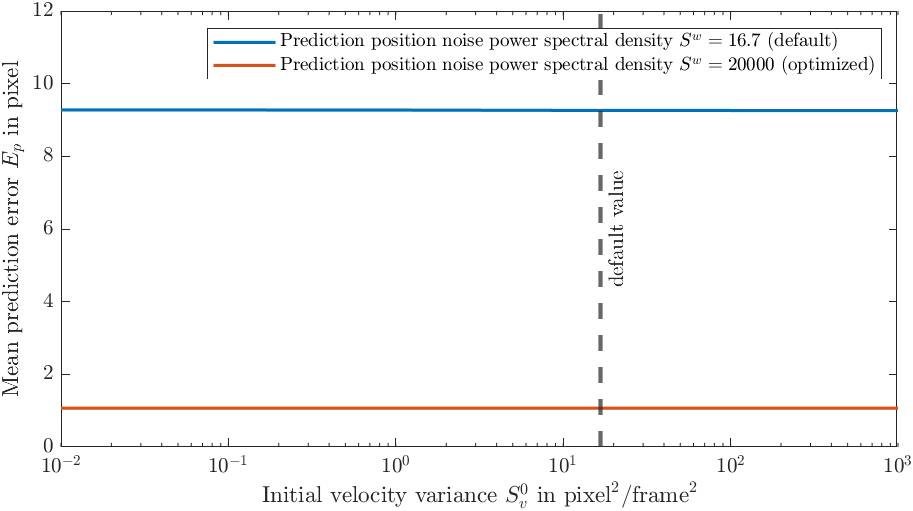
\includegraphics[width=\textwidth]{figures/KF/appendix/iniv cva.png}
		\caption{Initial velocity variance $S_{\mathrm{vel}}^{\mathrm{ini}}$ in CVA model.}
	\end{subfigure}
	\begin{subfigure}[t]{0.8\textwidth}
		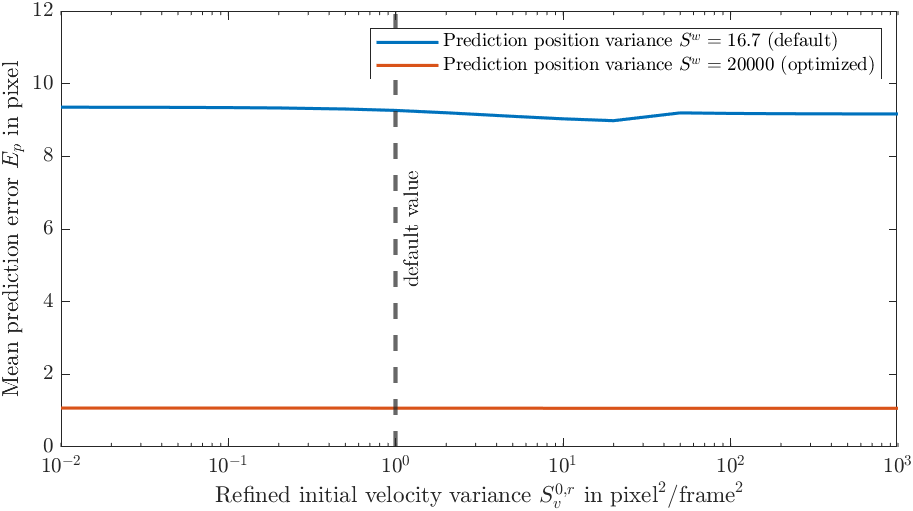
\includegraphics[width=\textwidth]{figures/KF/appendix/inirv cva.png}
		\caption{Refined initial velocity variance $S_{\mathrm{vel}}^{0,r}$ in CVA model.}
	\end{subfigure}
\end{figure}

\begin{figure}
    \ContinuedFloat
    \centering
	\begin{subfigure}[t]{0.8\textwidth}
		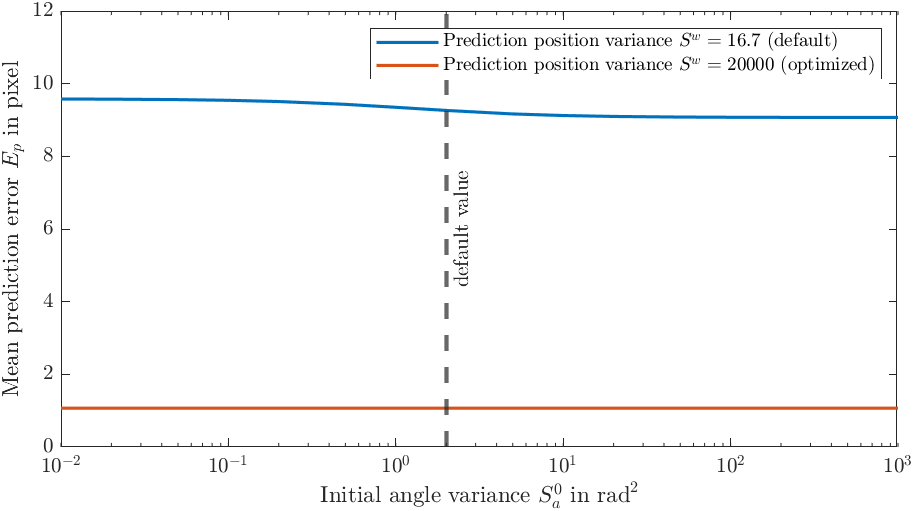
\includegraphics[width=\textwidth]{figures/KF/appendix/inia cva.png}
		\caption{Initial angle variance $S_{\mathrm{ang}}^{\mathrm{ini}}$ in CVA model.}
	\end{subfigure}
	\begin{subfigure}[t]{0.8\textwidth}
		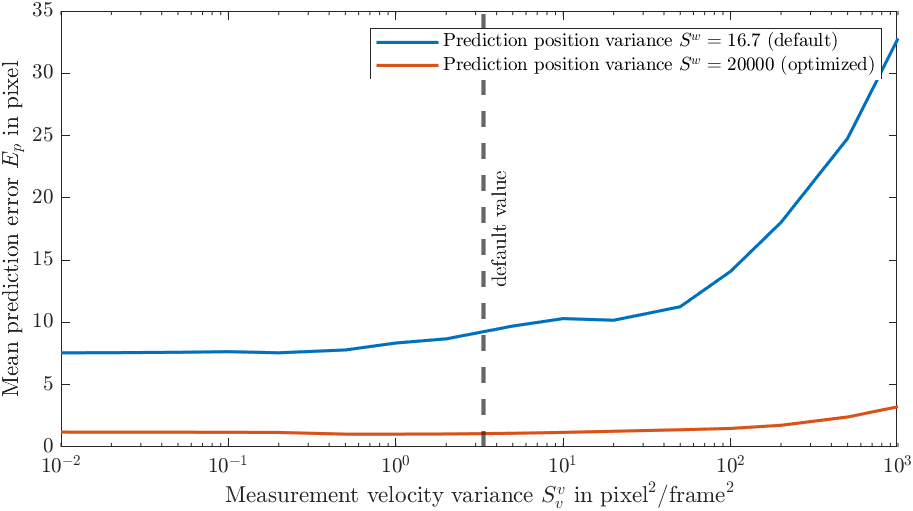
\includegraphics[width=\textwidth]{figures/KF/appendix/meav cva.png}
		\caption{Measurement velocity variance $S_{\mathrm{vel}}^{\boldsymbol{v}}$ in CVA model.}
	\end{subfigure}
	\begin{subfigure}[t]{0.8\textwidth}
		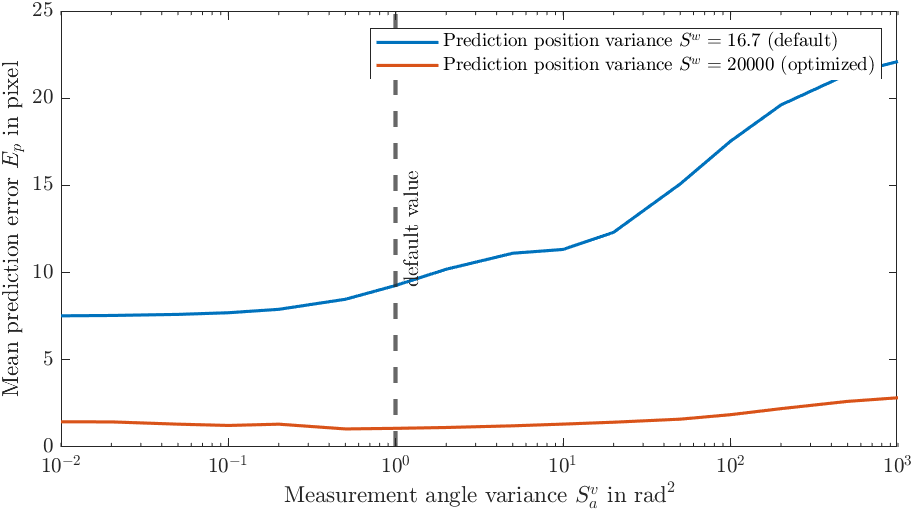
\includegraphics[width=\textwidth]{figures/KF/appendix/meaa cva.png}
		\caption{Measurement angle variance $S_{\mathrm{ang}}^{\boldsymbol{v}}$ in CVA model.}
	\end{subfigure}
\end{figure}

\begin{figure}
    \ContinuedFloat
    \centering
	\begin{subfigure}[t]{0.8\textwidth}
		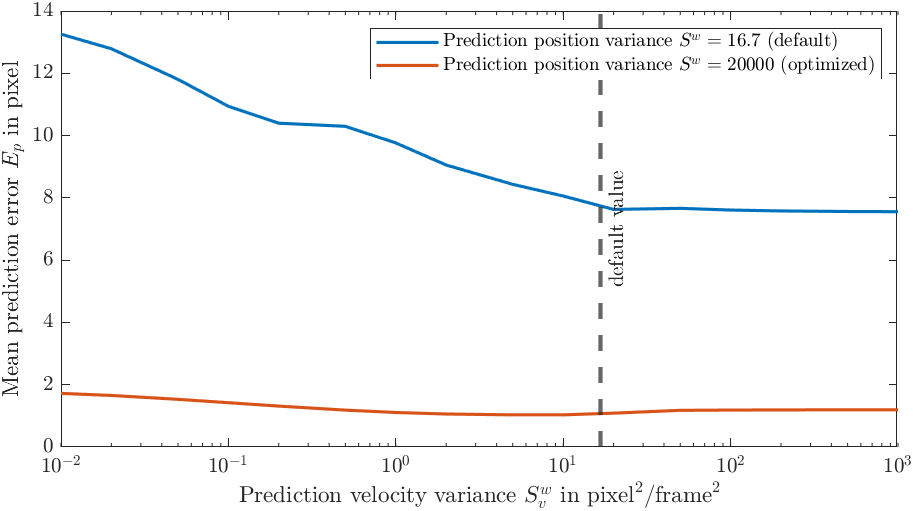
\includegraphics[width=\textwidth]{figures/KF/appendix/prev cva.png}
		\caption{Prediction velocity variance $S_{\mathrm{vel}}^{\boldsymbol{w}}$ in CVA model.}
	\end{subfigure}
	\begin{subfigure}[t]{0.8\textwidth}
		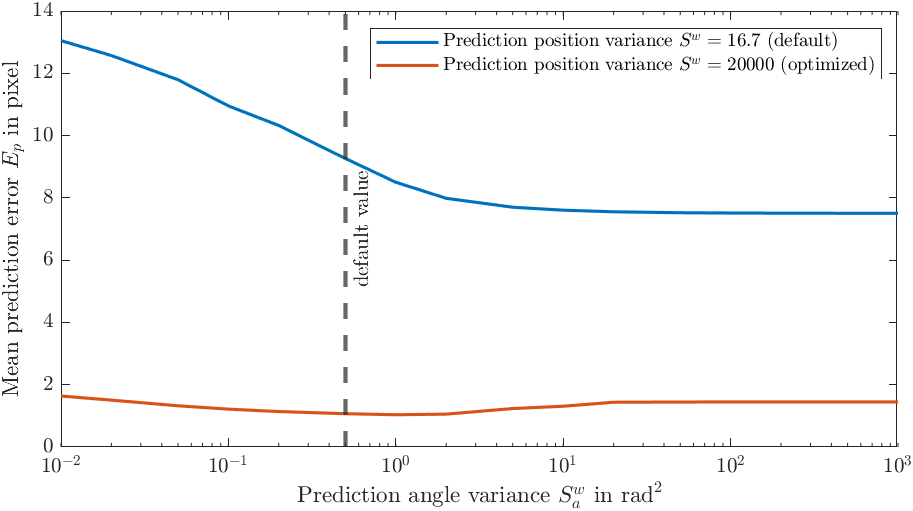
\includegraphics[width=\textwidth]{figures/KF/appendix/prea cva.png}
		\caption{Prediction angle variance $S_{\mathrm{ang}}^{\boldsymbol{w}}$ in CVA model.}
	\end{subfigure}
	\caption{The grid search result of each hyperparameters in CVA model when the prediction position noise power spectral density $S_{\mathrm{pos}}^{\boldsymbol{w}}$ is set as default or optimized value.}
	\label{grid search list}
\end{figure}

\begin{figure}[htbp]
    % \ContinuedFloat
	\centering
	\begin{subfigure}[t]{0.8\textwidth}
		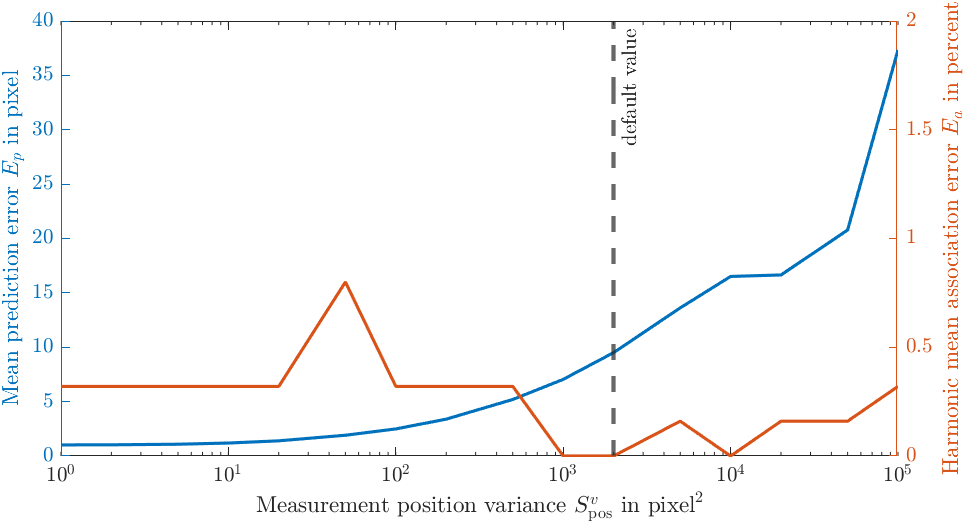
\includegraphics[width=\textwidth]{figures/KF/appendix/p cva meacov.png} 
		\caption{Measurement position noise power spectral density     $S_{\mathrm{pos}}^{\boldsymbol{v}}$ in CVA model with peppercorn dataset.}
	\end{subfigure}
	\vskip\baselineskip
	\quad
	\begin{subfigure}[t]{0.8\textwidth}
		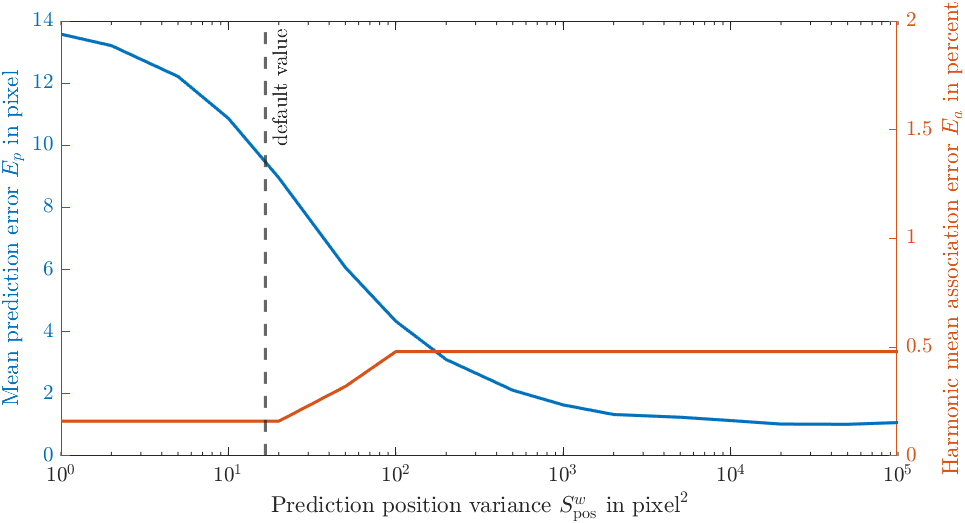
\includegraphics[width=\textwidth]{figures/KF/appendix/p cva precov.png}
		\caption{Prediction position noise power spectral density $S_{\mathrm{pos}}^{\boldsymbol{w}}$ in CVA model with peppercorn dataset.}
	\end{subfigure}
	\vskip\baselineskip
	\begin{subfigure}[t]{0.8\textwidth}
		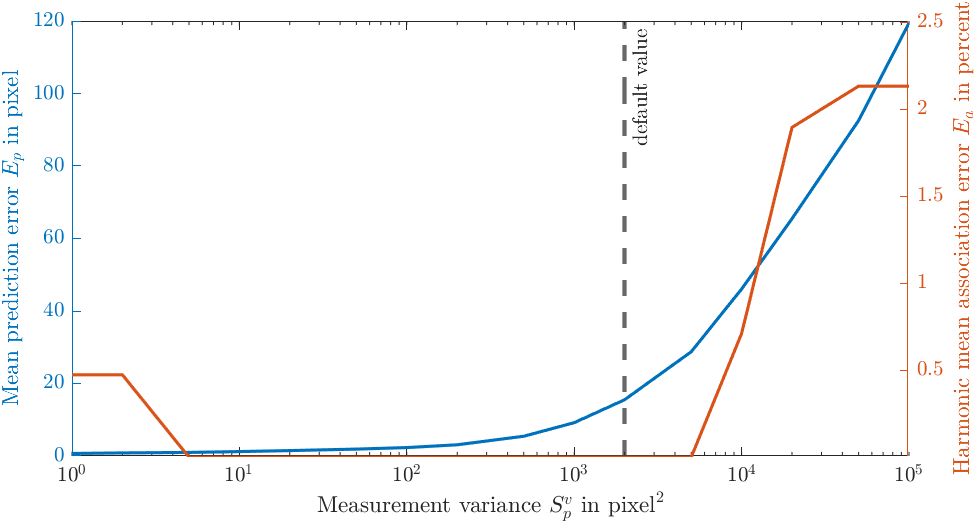
\includegraphics[width=\textwidth]{figures/KF/appendix/k cv meacov.png}
		\caption{Measurement noise power spectral density     $S^{\boldsymbol{v}}$ in CV model with sphere dataset.}
	\end{subfigure}
\end{figure}

\begin{figure}
    \ContinuedFloat
    \centering
	\begin{subfigure}[t]{0.8\textwidth}
		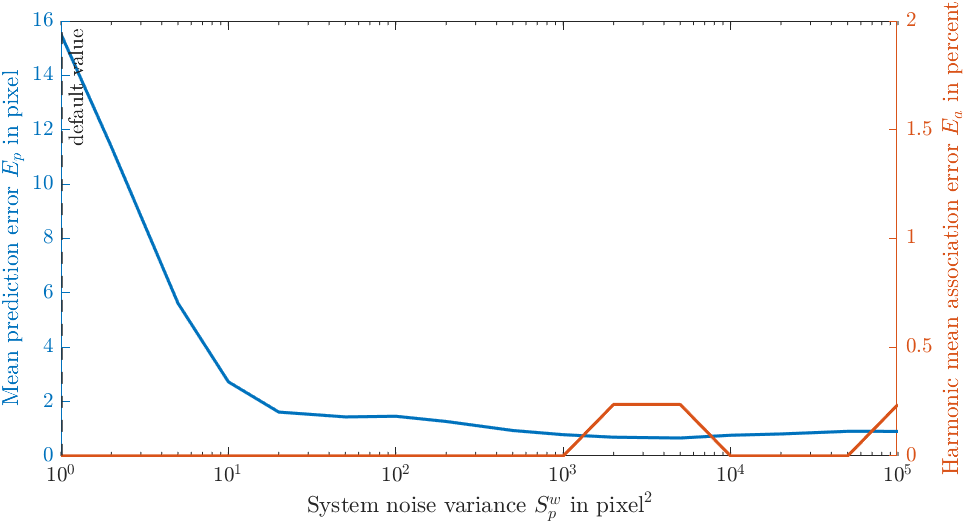
\includegraphics[width=\textwidth]{figures/KF/appendix/k cv precov.png}
		\caption{Prediction noise power spectral density     $S^{\boldsymbol{w}}$ in CV model with sphere dataset.}
	\end{subfigure}
	\begin{subfigure}[t]{0.8\textwidth}
		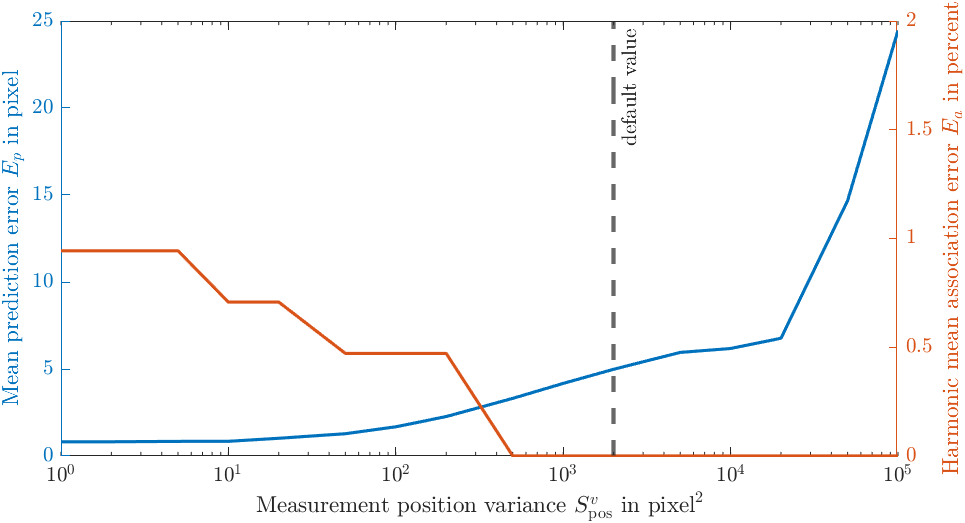
\includegraphics[width=\textwidth]{figures/KF/appendix/k cva meacov.png}
		\caption{Measurement position noise power spectral density     $S_{\mathrm{pos}}^{\boldsymbol{v}}$ in CVA model with sphere dataset.}
	\end{subfigure}
	\begin{subfigure}[t]{0.8\textwidth}
		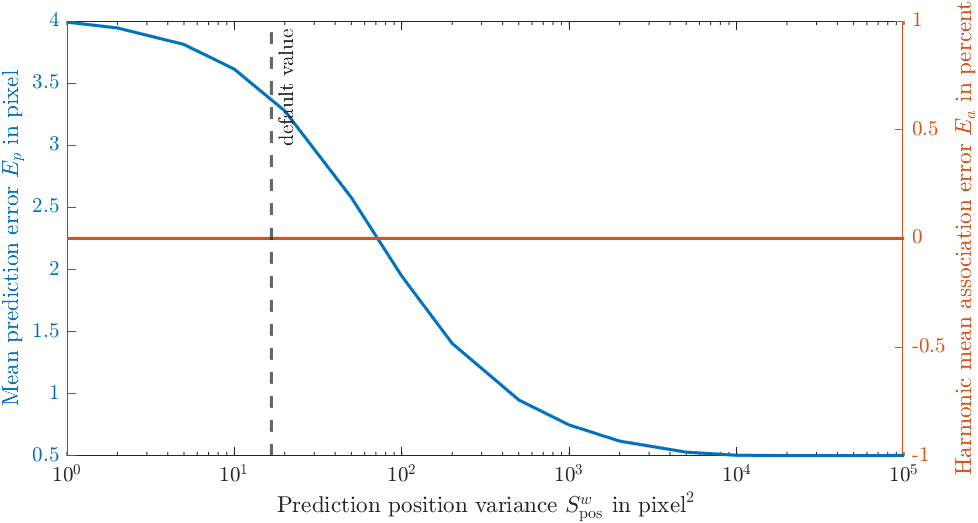
\includegraphics[width=\textwidth]{figures/KF/appendix/k cva precov.png}
		\caption{Prediction position noise power spectral density     $S_{\mathrm{pos}}^{\boldsymbol{w}}$ in CVA model with sphere dataset.}
	\end{subfigure}
\end{figure}

\begin{figure}
    \ContinuedFloat
    \centering
	\begin{subfigure}[t]{0.8\textwidth}
		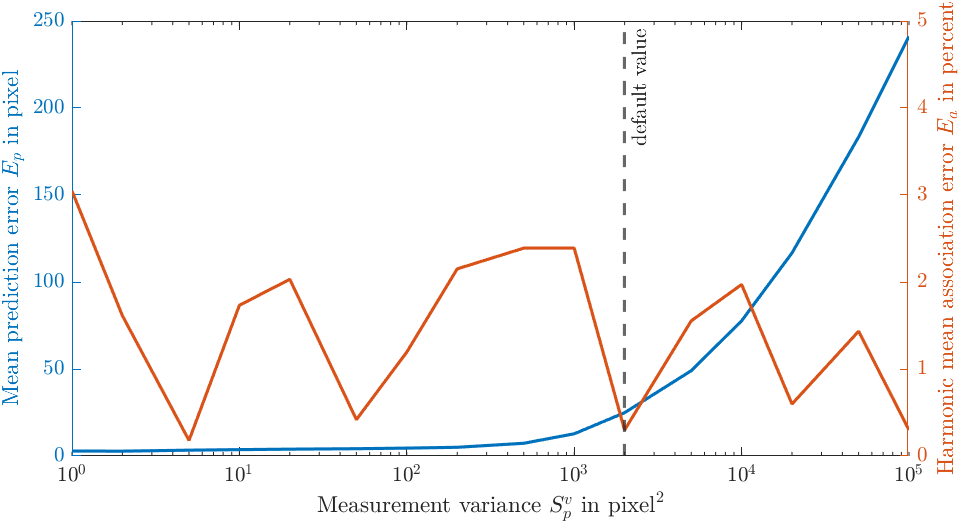
\includegraphics[width=\textwidth]{figures/KF/appendix/c cv meacov.png}
		\caption{Measurement noise power spectral density     $S^{\boldsymbol{v}}$ in CV model with cylinder dataset.}
	\end{subfigure}
	\begin{subfigure}[t]{0.8\textwidth}
		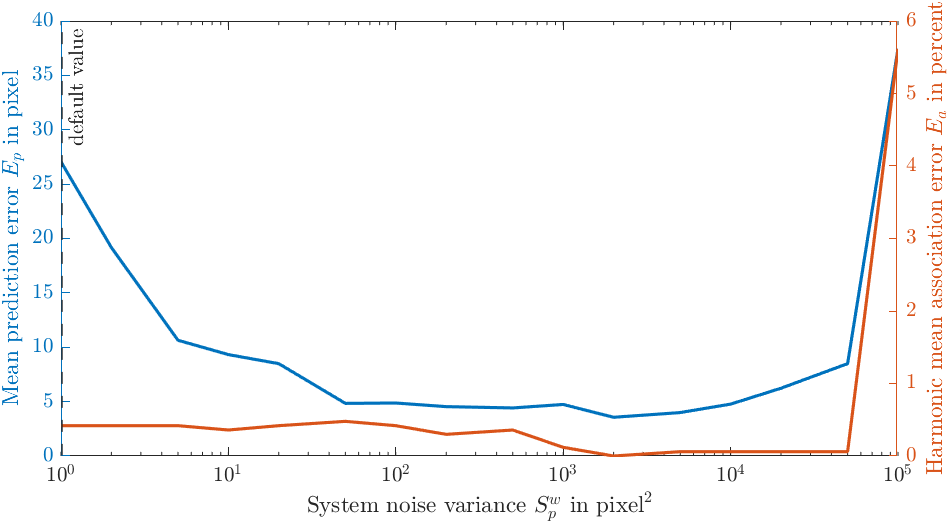
\includegraphics[width=\textwidth]{figures/KF/appendix/c cv precov.png}
		\caption{Prediction noise power spectral density     $S^{\boldsymbol{w}}$ in CV model with cylinder dataset.}
	\end{subfigure}
	\begin{subfigure}[t]{0.8\textwidth}
		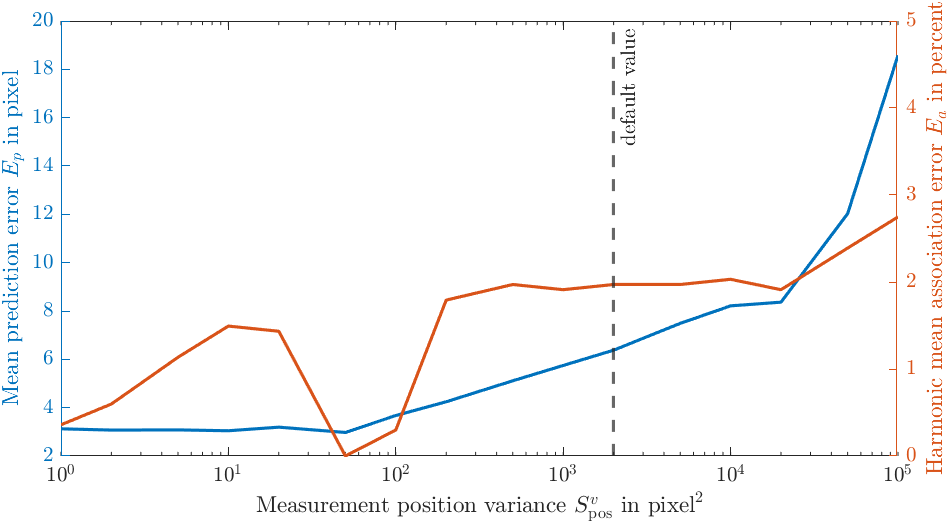
\includegraphics[width=\textwidth]{figures/KF/appendix/c cva meacov.png}
		\caption{Measurement position noise power spectral density     $S_{\mathrm{pos}}^{\boldsymbol{v}}$ in CVA model with cylinder dataset.}
	\end{subfigure}
\end{figure}

\begin{figure}
    \ContinuedFloat
    \centering
	\begin{subfigure}[t]{0.8\textwidth}
		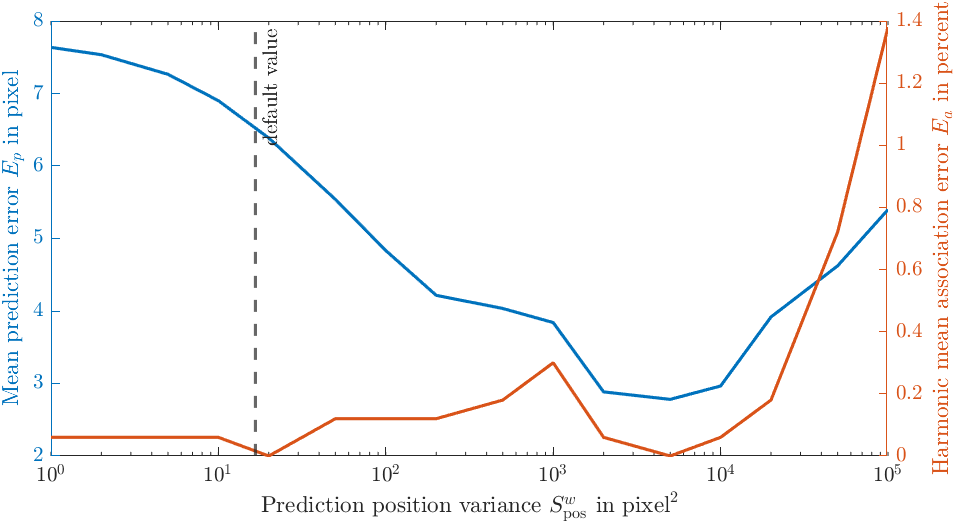
\includegraphics[width=\textwidth]{figures/KF/appendix/c cva precov.png}
		\caption{Prediction position noise power spectral density     $S_{\mathrm{pos}}^{\boldsymbol{w}}$ in CVA model with cylinder dataset.}
	\end{subfigure}
		\begin{subfigure}[t]{0.8\textwidth}
		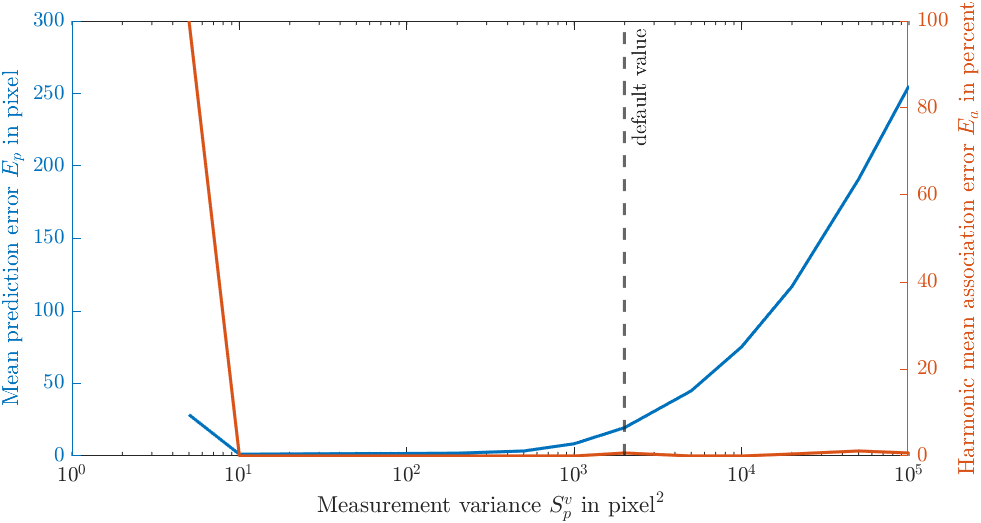
\includegraphics[width=\textwidth]{figures/KF/appendix/w cv meacov.png}
		\caption{Measurement noise power spectral density     $S^{\boldsymbol{v}}$ in CV model with wheat grain dataset.}
	\end{subfigure}
	\begin{subfigure}[t]{0.8\textwidth}
		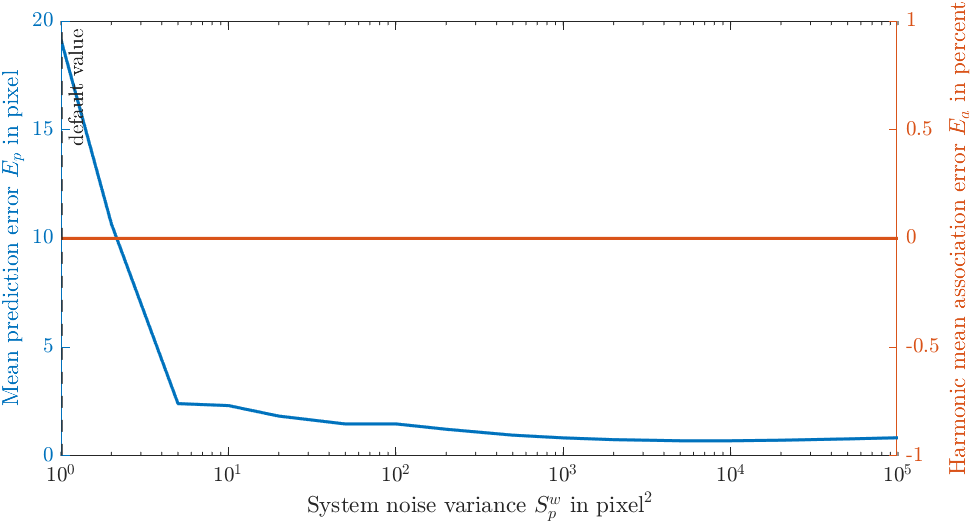
\includegraphics[width=\textwidth]{figures/KF/appendix/w cv precov.png}
		\caption{Prediction noise power spectral density     $S^{\boldsymbol{w}}$ in CV model with wheat grain dataset.}
	\end{subfigure}
\end{figure}

\begin{figure}
    \ContinuedFloat
    \centering
	\begin{subfigure}[t]{0.8\textwidth}
		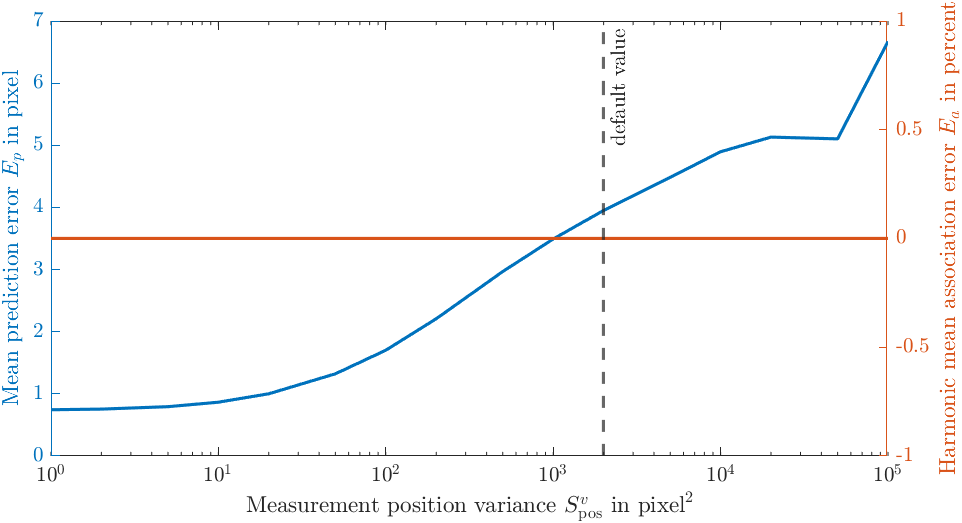
\includegraphics[width=\textwidth]{figures/KF/appendix/w cva meacov.png}
		\caption{Measurement position noise power spectral density     $S_{\mathrm{pos}}^{\boldsymbol{v}}$ in CVA model with wheat grain dataset.}
	\end{subfigure}
	\begin{subfigure}[t]{0.8\textwidth}
		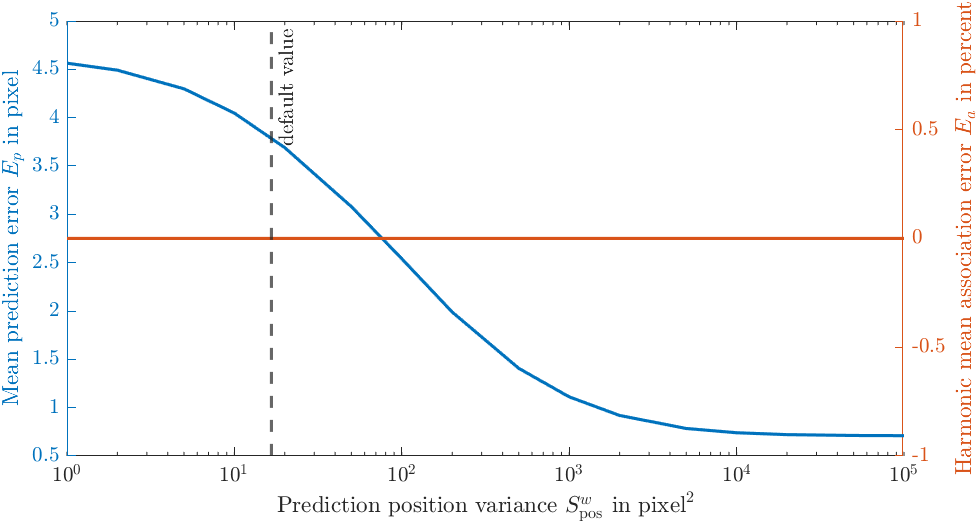
\includegraphics[width=\textwidth]{figures/KF/appendix/w cva precov.png}
		\caption{Prediction position noise power spectral density     $S_{\mathrm{pos}}^{\boldsymbol{w}}$ in CVA model with wheat grain dataset.}
	\end{subfigure}
	\caption{The grid search result of measurement and prediction noise power spectral density with other materials.}
	\label{grid search other material}
\end{figure}


\begin{figure}
    % \ContinuedFloat
    \centering
	\begin{subfigure}[t]{0.8\textwidth}
		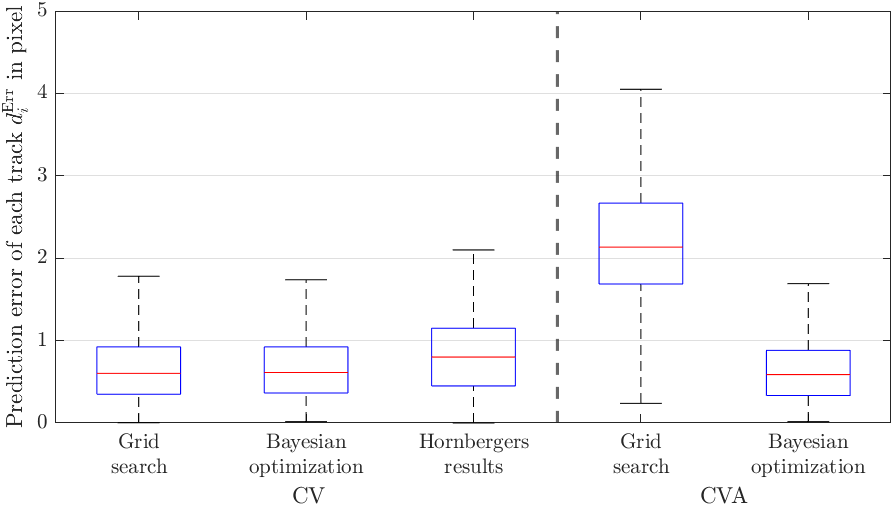
\includegraphics[width=\textwidth]{figures/KF/bayopt/effectOpt kugeln1.png}
		\caption{Comparison of the prediction error with the hyperparameters from different optimization methods with the sphere datasets.}
	\end{subfigure}
% 	\vskip\baselineskip
	\begin{subfigure}[t]{0.8\textwidth}
		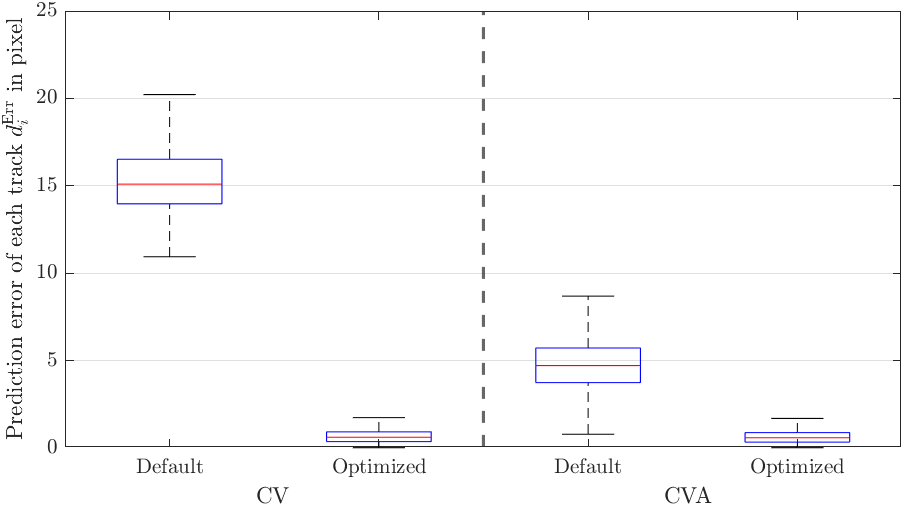
\includegraphics[width=\textwidth]{figures/KF/bayopt/effectOpt kugeln2.png}
		\caption{Comparison of the prediction error with the default and optimized hyperparameters with the sphere datasets.}
	\end{subfigure}
	\begin{subfigure}[t]{0.8\textwidth}
		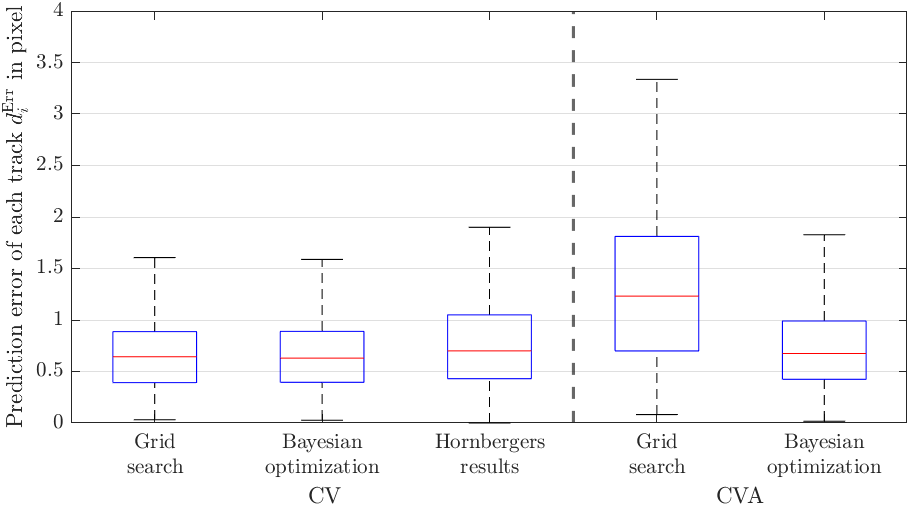
\includegraphics[width=\textwidth]{figures/KF/bayopt/effectOpt weizen1.png}
		\caption{Comparison of the prediction error with the hyperparameters from different optimization methods with the wheat grain datasets.}
	\end{subfigure}
\end{figure}

\begin{figure}
    \ContinuedFloat
    \centering
	\begin{subfigure}[t]{0.8\textwidth}
		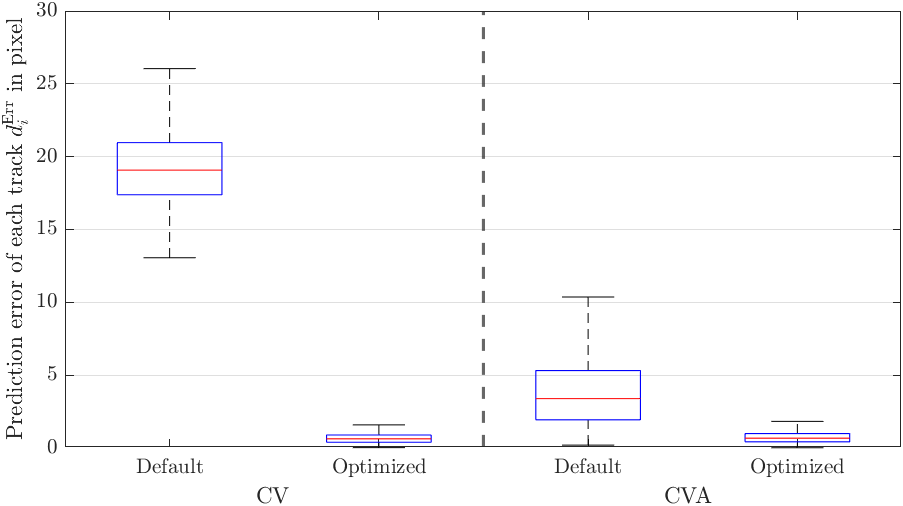
\includegraphics[width=\textwidth]{figures/KF/bayopt/effectOpt weizen2.png}
		\caption{Comparison of the prediction error with the default and optimized hyperparameters with the wheat grain datasets.}
	\end{subfigure}
% 	\vskip\baselineskip
	\begin{subfigure}[t]{0.8\textwidth}
		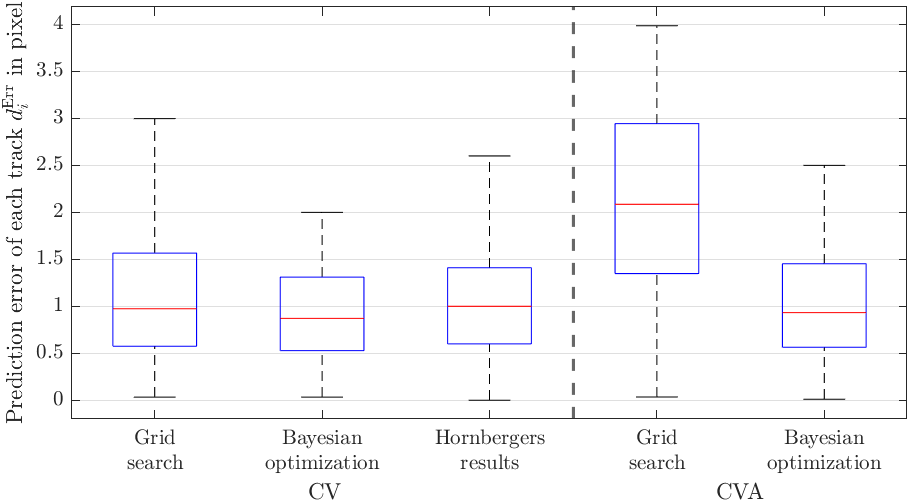
\includegraphics[width=\textwidth]{figures/KF/bayopt/effectOpt zylinder1.png}
		\caption{Comparison of the prediction error with the hyperparameters from different optimization methods with the cylinder datasets.}
	\end{subfigure}
	\begin{subfigure}[t]{0.8\textwidth}
		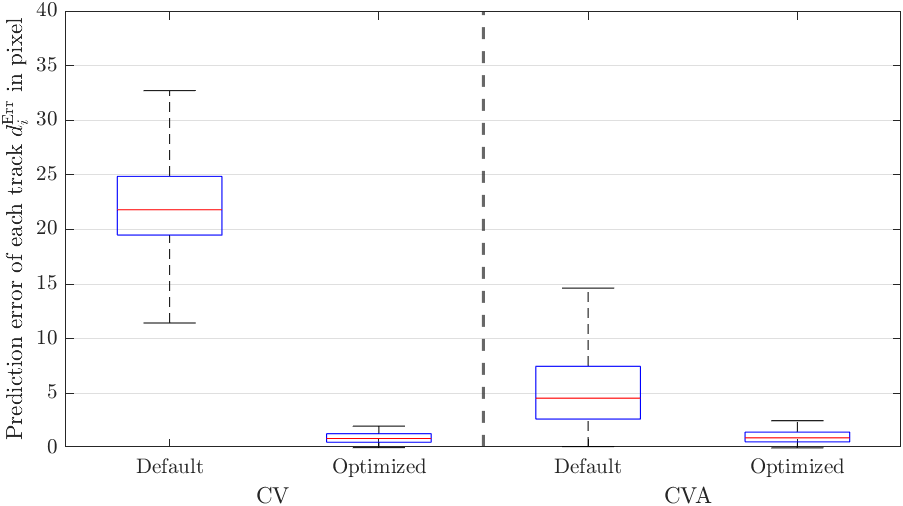
\includegraphics[width=\textwidth]{figures/KF/bayopt/effectOpt zylinder2.png}
		\caption{Comparison of the prediction error with the default and optimized hyperparameters with the cylinder datasets.}
	\end{subfigure}
\end{figure}

\begin{figure}
    \ContinuedFloat
    \centering
	\begin{subfigure}[t]{0.8\textwidth}
		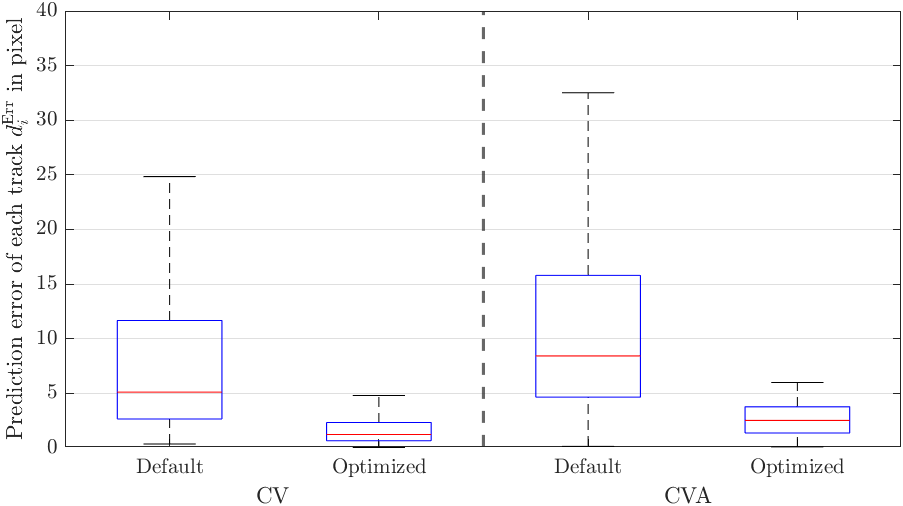
\includegraphics[width=\textwidth]{figures/KF/bayopt/effectOpt misch.png}
		\caption{Comparison of the prediction error with the default and optimized hyperparameters with the mixed material datasets.}
	\end{subfigure}
\end{figure}


\begin{figure}[htbp]
    % \ContinuedFloat
	\centering
	\begin{subfigure}[t]{0.75\textwidth}
		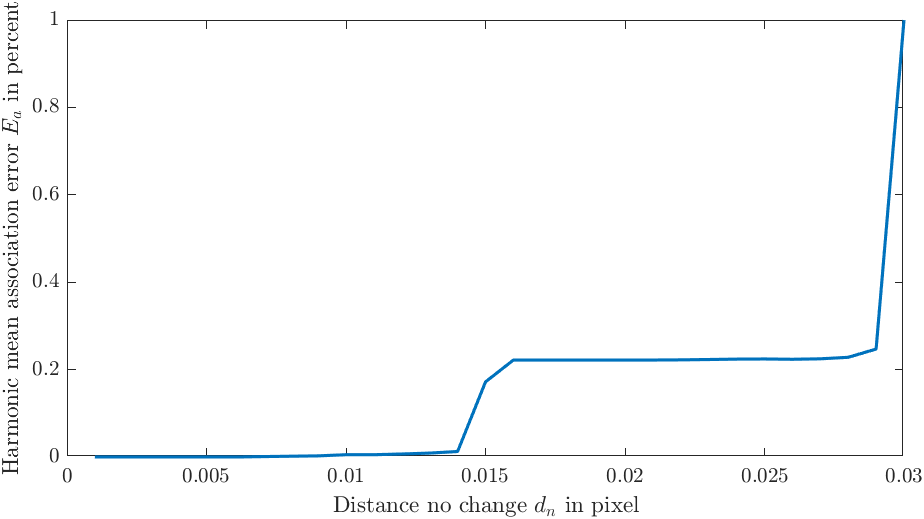
\includegraphics[width=\textwidth]{figures/Asso/gridsearch3.png} 
		\caption{Distance no change $d_{\mathrm{n}}$.}
	\end{subfigure}
	\vskip\baselineskip
	\quad
	\begin{subfigure}[t]{0.75\textwidth}
		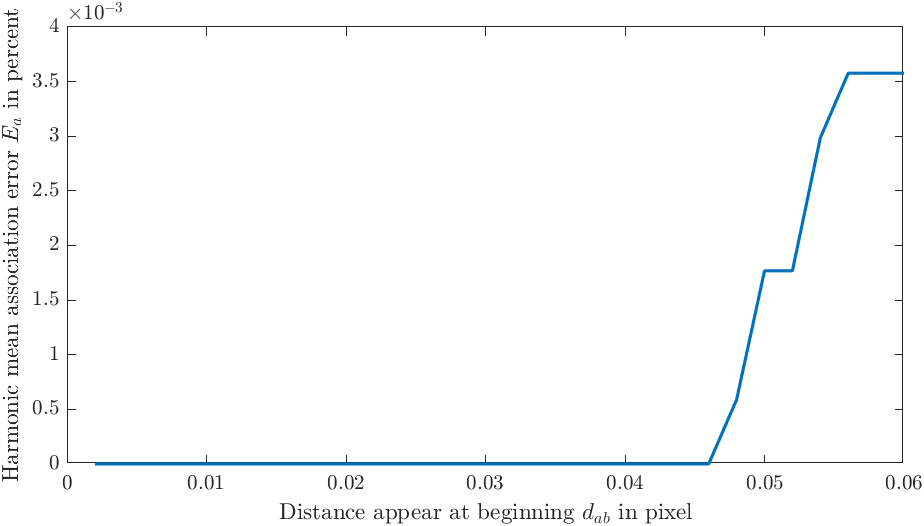
\includegraphics[width=\textwidth]{figures/Asso/gridsearch4.png}
		\caption{Distance appear at start $d_{\mathrm{as}}$.}
	\end{subfigure}
	\vskip\baselineskip
	\begin{subfigure}[t]{0.75\textwidth}
		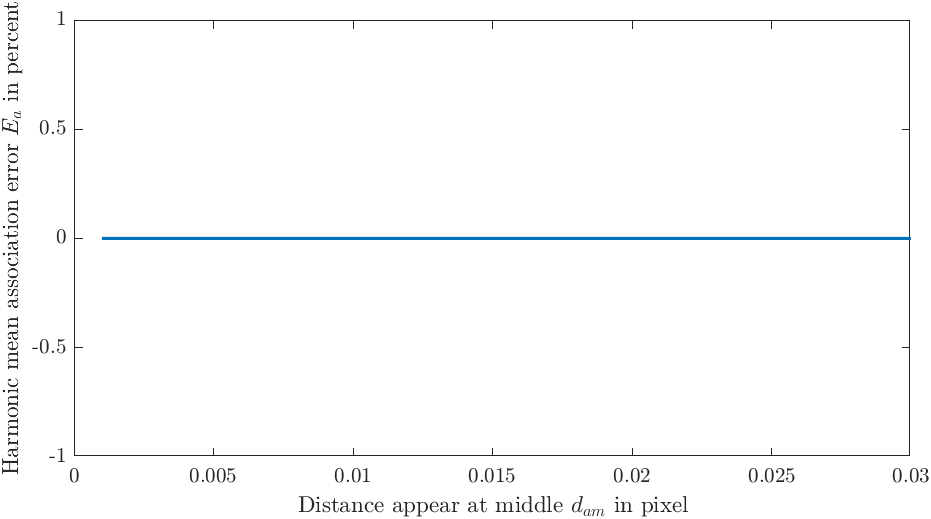
\includegraphics[width=\textwidth]{figures/Asso/gridsearch5.png}
		\caption{Distance appear at middle $d_{\mathrm{am}}$.}
	\end{subfigure}
	\caption{The grid search result of other association hyperparameters.}
	\label{grid search other}
\end{figure}

\begin{figure}[htbp]
    % \ContinuedFloat
	\centering
	\begin{subfigure}[t]{0.8\textwidth}
		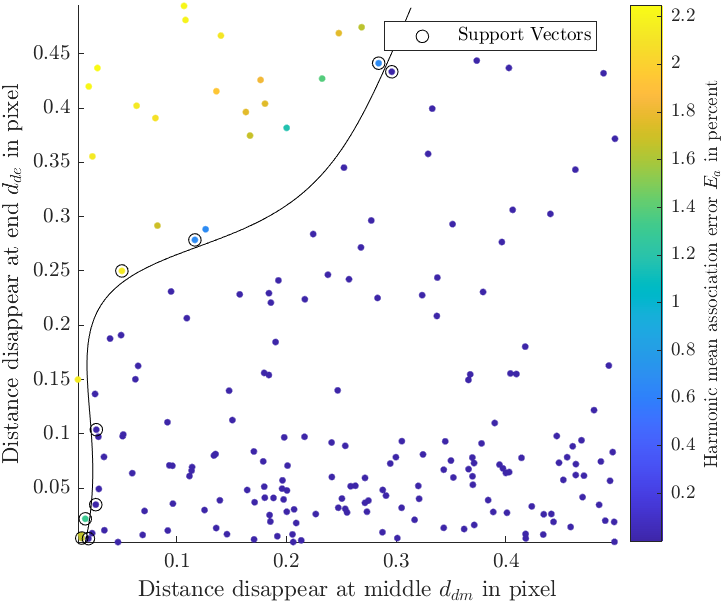
\includegraphics[width=\textwidth]{figures/Asso/svm01.png}
		\caption{Distance disappear at end $d_{\mathrm{de}}$ and distance disappear at middle $d_{\mathrm{dm}}$.}
	\end{subfigure}
	\vskip\baselineskip
	\quad
	\begin{subfigure}[t]{0.8\textwidth}
		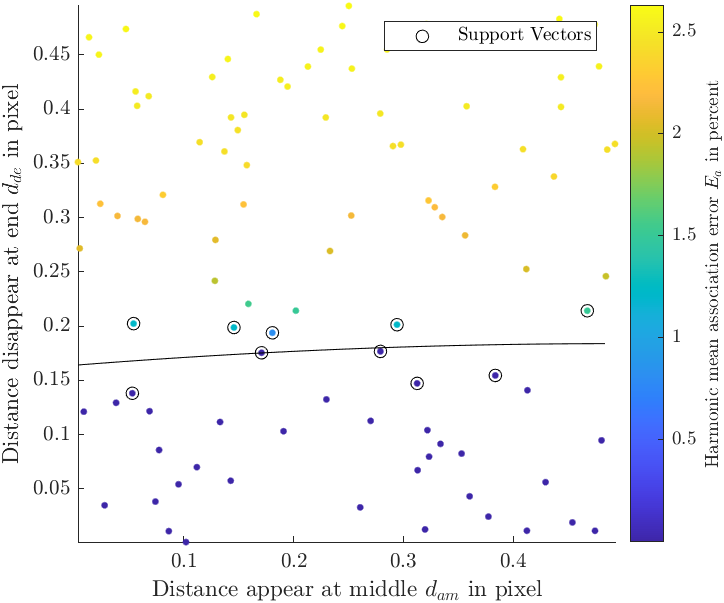
\includegraphics[width=\textwidth]{figures/Asso/svm02.png}
		\caption{Distance disappear at end $d_{\mathrm{de}}$ and distance appear at start $d_{\mathrm{as}}$.}
	\end{subfigure}
\end{figure}

\begin{figure}
    \ContinuedFloat
    \centering
	\begin{subfigure}[t]{0.8\textwidth}
		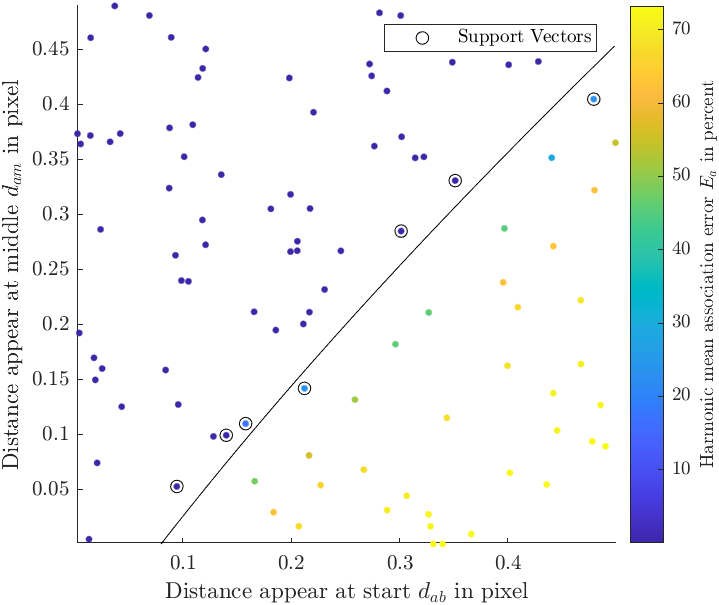
\includegraphics[width=\textwidth]{figures/Asso/svm03.png}
		\caption{Distance appear at middle $d_{\mathrm{am}}$ and distance appear at start $d_{\mathrm{as}}$}
	\end{subfigure}
	\caption{Some other 2-D SVM results.}
	\label{effect opt appendix}
\end{figure}







